\documentclass[11pt,a4paper]{article}

\usepackage[margin=2cm]{geometry}
\usepackage{microtype}
\usepackage{parskip}
\usepackage{enumitem}
\usepackage{graphicx}
\usepackage{caption}
\usepackage{rotating}
\usepackage[hidelinks]{hyperref}
\usepackage{titlesec}

\titleformat{\section}{\Large\bfseries}{}{0pt}{}
\titleformat{\subsection}{\large\bfseries}{}{0pt}{}

\captionsetup{labelfont=bf,font=small,skip=4pt}
\setlist[itemize]{leftmargin=1.5em,itemsep=0.2em,topsep=0.3em}

\title{Criterion B: Planning}
\author{}
\date{}

\begin{document}

\section*{Criterion B: Planning}

\subsection*{Decomposition}

I decomposed the problem into seven sub-systems mapped onto the CritA success criteria. Each sub-system passes through the full \emph{plan / design / develop / test / evaluate} cycle shown in the Gantt chart, and research blocks (Yjs CRDT semantics, Prisma schema patterns, JWT session security) are scheduled before the sub-systems that depend on them.

\begin{itemize}
  \item \textbf{Authentication} (SC1, SC9) --- registration, email verification via Resend, login, bcrypt password hashing, \texttt{httpOnly} JWT session cookies.
  \item \textbf{Workspace management} (SC3, SC4, SC7) --- create / rename / delete workspaces; public-vs-private visibility; collaborator invites; fork of public workspaces.
  \item \textbf{File management} (SC3, SC8) --- \texttt{.psc} / \texttt{.txt} CRUD inside a workspace; syntax-highlighted editor; mobile-responsive layout.
  \item \textbf{Pseudocode interpreter} (SC2) --- lexer, parser, async executor handling \texttt{input}\,/\,\texttt{output}, runtime error reporting with line numbers.
  \item \textbf{Realtime co-editing} (SC5) --- Yjs CRDT document per file, authenticated WebSocket transport, presence via awareness, debounced server-side flush.
  \item \textbf{Version control} (SC6) --- per-file \texttt{FileVersion} rows on each save, line-level diff UI, restore, named-commit option.
  \item \textbf{Platform \& performance} (SC10) --- Next.js on Vercel, dedicated WebSocket server on Fly.io, Neon Postgres, dashboard load $\leq 3$\,s.
\end{itemize}

The final fortnight (April 2026) is reserved for integration testing across sub-systems, mobile-viewport regression, and writing the CritE evaluation against the success criteria.

\begin{figure}[h]
  \centering
  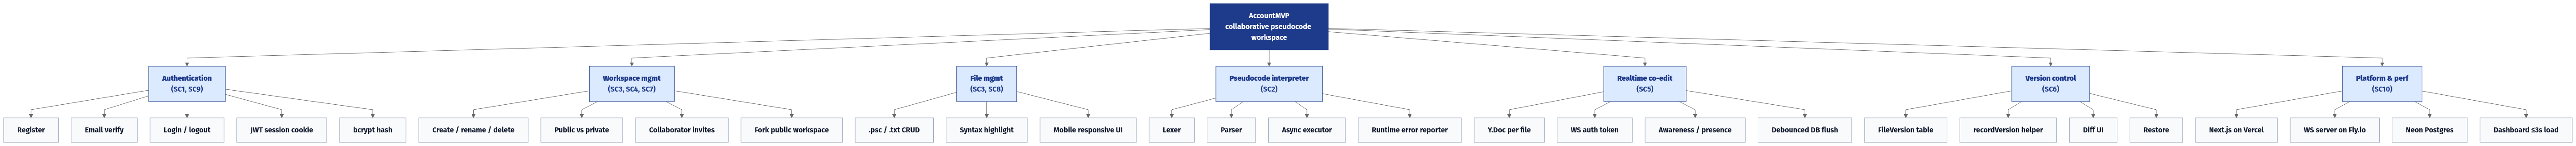
\includegraphics[width=\textwidth,keepaspectratio]{diagrams/structure_chart.png}
  \caption{Structure chart: the seven sub-systems decomposed into concrete modules. Each leaf maps to a unit of work in the Gantt chart.}
\end{figure}

\clearpage

\begin{figure}[h]
  \centering
  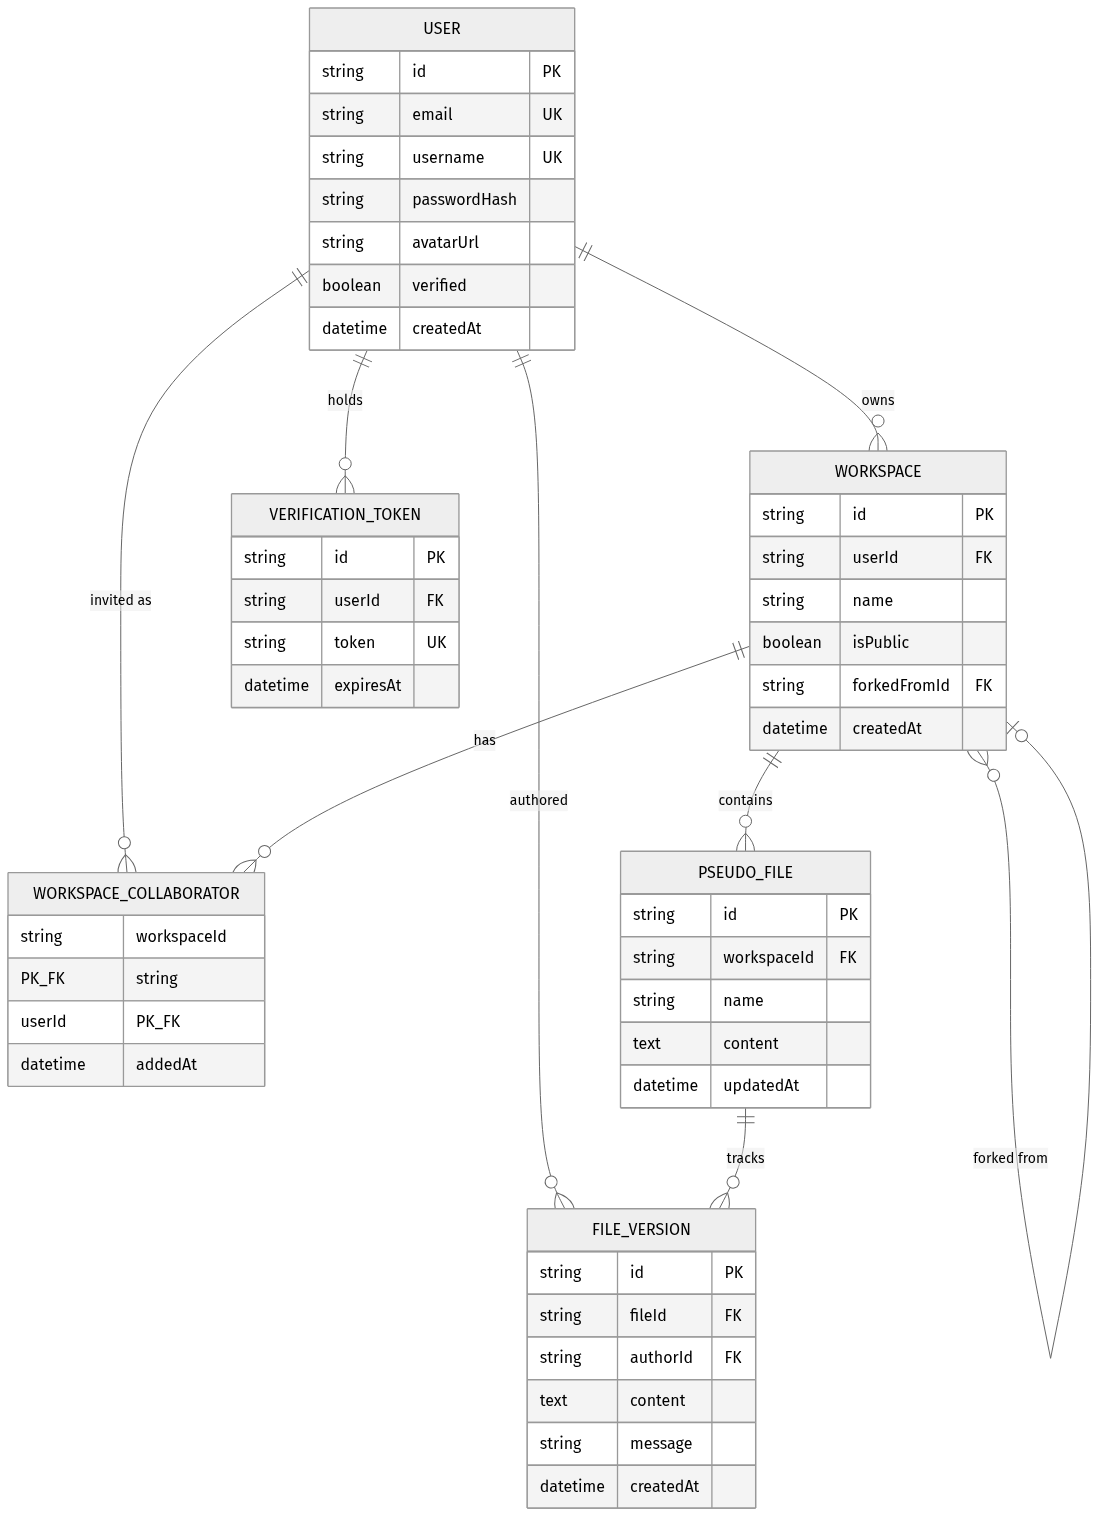
\includegraphics[width=\textwidth,keepaspectratio]{diagrams/erd.png}
  \caption{Entity-relationship diagram of the Postgres schema backing persistence. \texttt{Workspace} has a self-referential \texttt{forkedFromId} edge for fork lineage; \texttt{FileVersion} captures author attribution required by the version-control sub-system.}
\end{figure}

\subsection*{Gantt chart}

\begin{sidewaysfigure}
  \centering
  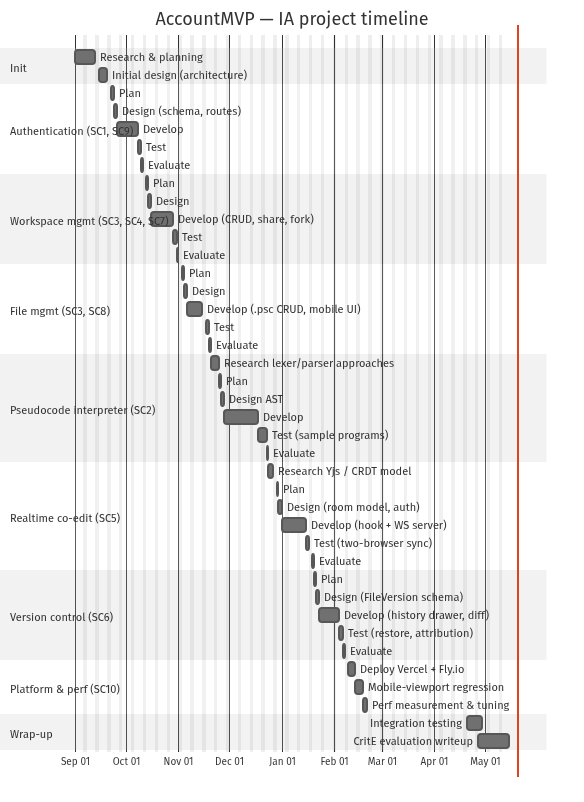
\includegraphics[width=0.95\textheight,keepaspectratio]{diagrams/gantt.png}
  \caption{Gantt chart covering every sub-system through plan, design, develop, test, and evaluate. Research blocks precede the sub-systems that depend on them. Wrap-up (integration + evaluation writeup) occupies the final three weeks.}
\end{sidewaysfigure}

\end{document}
